\section{Linear First Order Equations}

\noindent
A first order differential equation is said to be {\color{blue}\it linear\/} if it can be written as

\begin{equation}
  \label{eq:2.1.1}y'+p(x)y=f(x).
\end{equation}
A first order differential equation that can't be written like this is {\color{blue}\it
nonlinear\/}. We say that \eqref{eq:2.1.1} is {\color{blue}\it homogeneous\/} if $f\equiv0$;
otherwise it's {\color{blue}\it nonhomogeneous\/}. Since $y\equiv0$ is obviously a solution of the
homogeneous equation
\[
  y'+p(x)y=0,
\]
we call it the {\color{blue}\it trivial solution\/}. Any other solution is {\color{blue}\it
nontrivial\/}.

\begin{example}
  \label{example:2.1.1}\rm The first order equations
  \begin{eqnarray*}
    x^{2}y'+3y   & = & x^{2},  \\[2\jot]
    xy'-8x^{2}y  & = & \sin x, \\
    xy'+(\ln x)y & = & 0,      \\
    y'           & = & x^{2}y-2,
  \end{eqnarray*}
  are not in the form \eqref{eq:2.1.1}, but they are linear, since they can be rewritten as
  \begin{eqnarray*}
    y'+\frac{3}{x^{2}}y & = & 1,                \\
    y'-8xy              & = & \frac{\sin x}{x}, \\
    y'+\frac{\ln x}{x}y & = & 0,                \\
    y'-x^{2}y           & = & -2.
  \end{eqnarray*}
\end{example}
% no solution

\begin{example}
  \label{example:2.1.2}\rm Here are some nonlinear first order equations:
  \[
    \begin{array}{rcrc}
      xy'+3y^{2} & = & 2x & \qquad\mbox{(because $y$ is squared)},       \\[2\jot]
      yy'        & = & 3  & \qquad\mbox{(because of the product $yy'$)}, \\[2\jot]
      y'+xe^{y}  & = & 12 & \qquad\mbox{(because of $e^{y}$)}.
    \end{array}
  \]
\end{example}
% no solution

\boxit{General Solution of a Linear First Order Equation}

\noindent
To motivate a definition that we'll need, consider the simple linear first order equation
\begin{equation}
  \label{eq:2.1.2}y'=\frac{1}{x^{2}}.
\end{equation}
From calculus we know that $y$ satisfies this equation if and only if
\begin{equation}
  \label{eq:2.1.3}y=-\frac{1}{x}+c,
\end{equation}
where $c$ is an arbitrary constant. We call $c$ a {\color{blue}\it parameter\/} and say that
\eqref{eq:2.1.3} defines a {\color{blue}\it one--parameter family\/} of functions. For each real
number $c$, the function defined by \eqref{eq:2.1.3} is a solution of \eqref{eq:2.1.2} on
$(-\infty,0)$ and $(0,\infty)$; moreover, every solution of \eqref{eq:2.1.2} on either of these
intervals is of the form \eqref{eq:2.1.3} for some choice of $c$. We say that \eqref{eq:2.1.3} is
{\color{blue}\it the general solution\/} of~\eqref{eq:2.1.2}.

We'll see that a similar situation occurs in connection with any first order linear equation
\begin{equation}
  \label{eq:2.1.4}y'+p(x)y=f(x);
\end{equation}
that is, if $p$ and $f$ are continuous on some open interval $(a,b)$ then there's a unique formula
$y=y(x,c)$ analogous to \eqref{eq:2.1.3} that involves $x$ and a parameter $c$ and has these
properties:
\begin{itemize}
  \item % (a)
    For each fixed value of $c$, the resulting function of $x$ is a solution of \eqref{eq:2.1.4} on
    $(a,b)$.

  \item % (b)
    If $y$ is a solution of \eqref{eq:2.1.4} on $(a,b)$, then $y$ can be obtained from the formula
    by choosing $c$ appropriately.
\end{itemize}
We'll call $y=y(x,c)$ the {\color{blue}\it general solution\/} of \eqref{eq:2.1.4}.

When this has been established, it will follow that an equation of the form
\begin{equation}
  \label{eq:2.1.5}P_{0}(x)y'+P_{1}(x)y=F(x)
\end{equation}
has a general solution on any open interval $(a,b)$ on which $P_{0}$, $P_{1}$, and $F$ are all
continuous and $P_{0}$ has no zeros, since in this case we can rewrite \eqref{eq:2.1.5} in the form
\eqref{eq:2.1.4} with $p=P_{1}/P_{0}$ and $f=F/P_{0}$, which are both continuous on $(a,b)$.

To avoid awkward wording in examples and exercises, we won't specify the interval $(a,b)$ when we
ask for the general solution of a specific linear first order equation. Let's agree that this always
means that we want the general solution on every open interval on which $p$ and $f$ are continuous
if the equation is of the form \eqref{eq:2.1.4}, or on which $P_{0}$, $P_{1}$, and $F$ are
continuous and $P_{0}$ has no zeros, if the equation is of the form \eqref{eq:2.1.5}. We leave it to
you to identify these intervals in specific examples and exercises.

For completeness, we point out that if $P_{0}$, $P_{1}$, and $F$ are all continuous on an open
interval $(a,b)$, but $P_{0}$ {\color{blue}\it does\/} have a zero in $(a,b)$, then \eqref{eq:2.1.5}
may fail to have a general solution on $(a,b)$ in the sense just defined. Since this isn't a major
point that needs to be developed in depth, we won't discuss it further; however, see
Exercise~\ref{exer:2.1.44} for an example.

\boxit{Homogeneous Linear First Order Equations}

\noindent
We begin with the problem of finding the general solution of a homogeneous linear first order
equation. The next example recalls a familiar result from calculus.

\begin{example}
  \label{example:2.1.3} \rm Let $a$ be a constant.
  \begin{alist}
    \item % (a)
    Find the general solution of
    \begin{equation}
      y'-ay=0.\label{eq:2.1.6}
    \end{equation}

    \item % (b)
    Solve the initial value problem
    \[
      y'-ay=0,\quad y(x_{0})=y_{0}.
    \]
  \end{alist}
\end{example}

\begin{examplesolution}
\solutionpart{a} You already know from calculus that if $c$ is any constant, then $y=ce^{ax}$
satisfies \eqref{eq:2.1.6}. However, let's pretend you've forgotten this, and use this problem to
illustrate a general method for solving a homogeneous linear first order equation.

We know that \eqref{eq:2.1.6} has the trivial solution $y\equiv0$. Now suppose $y$ is a nontrivial
solution of \eqref{eq:2.1.6}. Then, since a differentiable function must be continuous, there must
be some open interval $I$ on which $y$ has no zeros. We rewrite \eqref{eq:2.1.6} as
\[
  \frac{y'}{y}=a
\]
for $x$ in $I$. Integrating this shows that
\[
  \ln|y|=ax+k,\mbox{\quad so \quad}|y|=e^{k}e^{ax},
\]
where $k$ is an arbitrary constant. Since $e^{ax}$ can never equal zero, $y$ has no zeros, so $y$ is
either always positive or always negative. Therefore we can rewrite $y$ as
\begin{equation}
  \label{eq:2.1.7}y=ce^{ax}
\end{equation}
where
\[
  c=\left\{
  \begin{array}{cl}
    \phantom{-}e^{k} & \mbox{if }y>0, \\
    -e^{k}           & \mbox{if }y<0.
  \end{array}\right.
\]
This shows that every nontrivial solution of \eqref{eq:2.1.6} is of the form $y=ce^{ax}$ for some
nonzero constant $c$. Since setting $c=0$ yields the trivial solution, {\color{blue}\it all\/}
solutions of \eqref{eq:2.1.6} are of the form \eqref{eq:2.1.7}. Conversely, \eqref{eq:2.1.7} is a
solution of \eqref{eq:2.1.6} for every choice of $c$, since differentiating \eqref{eq:2.1.7} yields
$y'=ace^{ax}=ay$.

\solutionpart{b} Imposing the initial condition $y(x_{0})=y_{0}$ yields $y_{0}=ce^{ax_{0}}$, so
$c=y_{0}e^{-ax_{0}}$ and
\[
  y=y_{0}e^{-ax_{0}}e^{ax}=y_{0}e^{a(x-x_{0})}.
\]
Figure~\ref{figure:2.1.1} shows the graphs of this function with $x_{0}=0$, $y_{0}=1$, and various
values of $a$.

\begin{figure}[tbp]
  \centering
  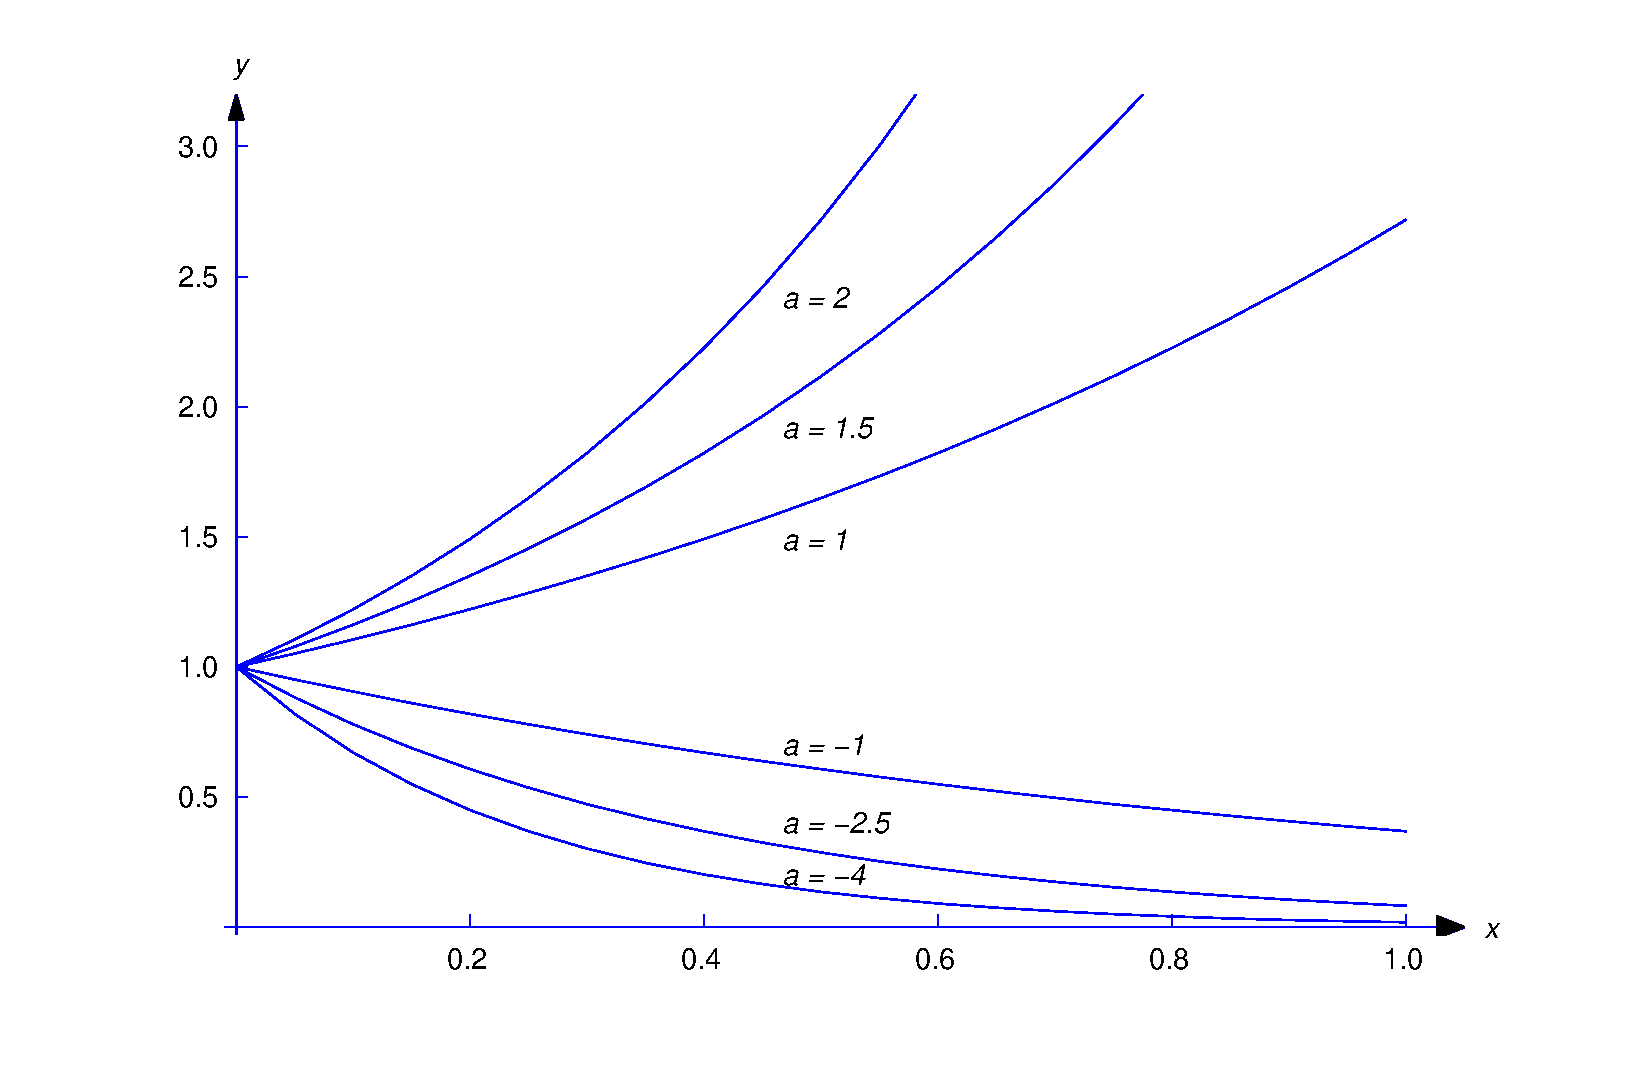
\includegraphics[bb=-78 148 689 643, width=5.67in, height=3.66in, keepaspectratio]{fig020101}
  \color{blue}
  \caption{Solutions of $y'-ay=0$, $y(0)=1$}
  \label{figure:2.1.1}
\end{figure}
\end{examplesolution}

\begin{example}
  \label{example:2.1.4}\rm

  \begin{alist}
    \item % (a)
    Find the general solution of
    \begin{equation}
      xy'+y=0.\label{eq:2.1.8}
    \end{equation}

    \item % (b)
    Solve the initial value problem
    \begin{equation}
      xy'+y=0,\quad y(1)=3.\label{eq:2.1.9}
    \end{equation}
  \end{alist}
\end{example}

\begin{examplesolution}
\solutionpart{a} We rewrite \eqref{eq:2.1.8} as
\begin{equation}
  \label{eq:2.1.10}y'+\frac{1}{x}y=0,
\end{equation}
where $x$ is restricted to either $(-\infty,0)$ or $(0,\infty)$. If $y$ is a nontrivial solution of
\eqref{eq:2.1.10}, there must be some open interval I on which $y$ has no zeros. We can rewrite
\eqref{eq:2.1.10} as
\[
  \frac{y'}{y}=-\frac{1}{x}
\]
for $x$ in $I$. Integrating shows that
\[
  \ln|y|=-\ln|x|+k,\mbox{\quad so\quad}|y|=\frac{e^{k}}{|x|}.
\]
Since a function that satisfies the last equation can't change sign on either $(-\infty,0)$ or
$(0,\infty)$, we can rewrite this result more simply as
\begin{equation}
  \label{eq:2.1.11}y=\frac{c}{x}
\end{equation}
where
\[
  c=\left\{
  \begin{array}{cl}
    \phantom{-}e^{k} & \mbox{if }y>0, \\
    -e^{k}           & \mbox{if }y<0.
  \end{array}\right.
\]
We've now shown that every solution of \eqref{eq:2.1.10} is given by \eqref{eq:2.1.11} for some
choice of $c$. (Even though we assumed that $y$ was nontrivial to derive \eqref{eq:2.1.11}, we can
get the trivial solution by setting $c=0$ in \eqref{eq:2.1.11}.) Conversely, any function of the
form \eqref{eq:2.1.11} is a solution of \eqref{eq:2.1.10}, since differentiating \eqref{eq:2.1.11}
yields
\[
  y'=-\frac{c}{x^{2}},
\]
and substituting this and \eqref{eq:2.1.11} into \eqref{eq:2.1.10} yields
\begin{eqnarray*}
  y'+\frac{1}{x}y & = & -\frac{c}{x^{2}}+\frac{1}{x}\frac{c}{x} \\[2\jot]
                  & = & -\frac{c}{x^{2}}+\frac{c}{x^{2}}=0.
\end{eqnarray*}

Figure~\ref{figure:2.1.2} shows the graphs of some solutions corresponding to various values of $c$. \solutionpart{b} Imposing the initial condition $y(1)=3$ in \eqref{eq:2.1.11} yields $c=3$.
Therefore the solution of \eqref{eq:2.1.9} is
\[
  y=\frac{3}{x}.
\]
The interval of validity of this solution is $(0,\infty)$.

\begin{figure}[tbp]
  \centering
  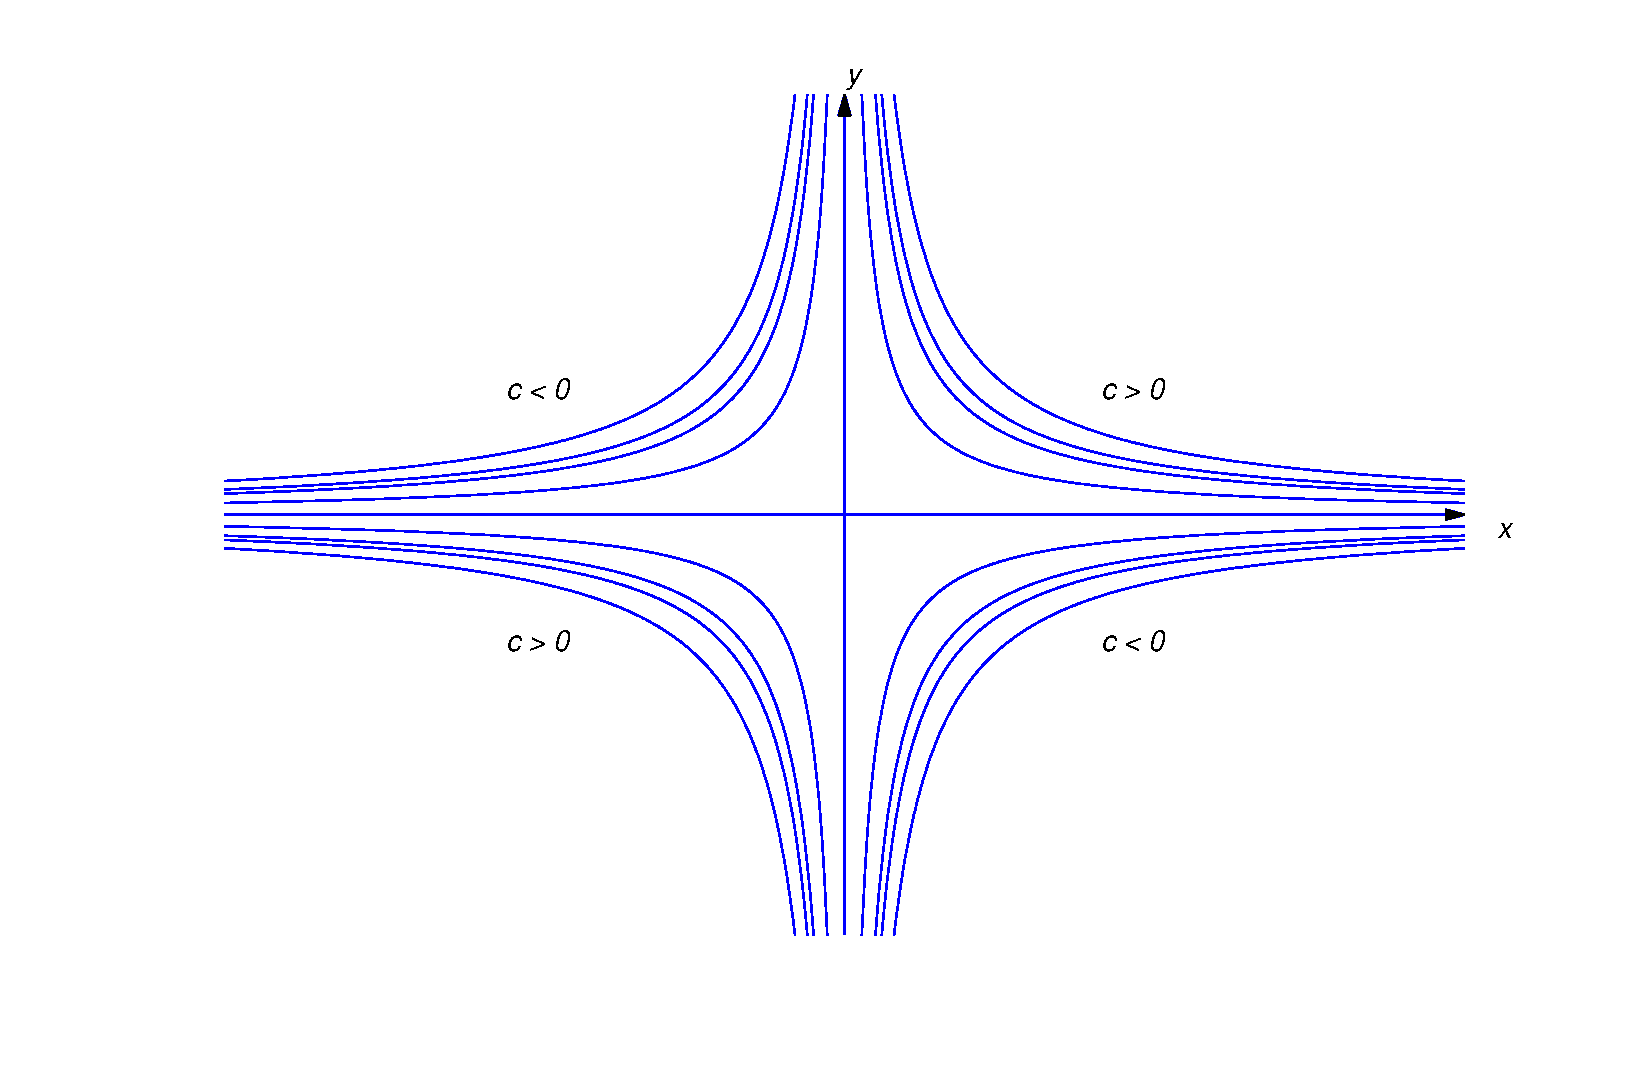
\includegraphics[bb=-78 148 689 643, width=5.67in, height=3.66in, keepaspectratio]{fig020102}
  \color{blue}
  \caption{Solutions of $xy'+y=0$ on $(0,\infty)$ and $(-\infty,0)$}
  \label{figure:2.1.2}
\end{figure}
\end{examplesolution}

The results in Examples~\ref{example:2.1.3}\part{a} and \ref{example:2.1.4}\part{a} are special
cases of the next theorem.

\begin{theorem}
  \color{blue}
  \label{thmtype:2.1.1} If $p$ is continuous on $(a,b)$, then the general solution of the
  homogeneous equation
  \begin{equation}
    \label{eq:2.1.12}y'+p(x)y=0
  \end{equation}
  on $(a,b)$ is
  \[
    y=ce^{-P(x)},
  \]
  where
  \begin{equation}
    \label{eq:2.1.13}P(x)=\int p(x)\,dx
  \end{equation}
  is any antiderivative of $p$ on $(a,b)$; that is,
  \begin{equation}
    \label{eq:2.1.14}P'(x)=p(x),\quad a<x<b.
  \end{equation}
\end{theorem}

\proof If $y=ce^{-P(x)}$, differentiating $y$ and using \eqref{eq:2.1.14} shows that
\[
  y'=-P'(x)ce^{-P(x)}=-p(x)ce^{-P(x)}=-p(x)y,
\]
so $y'+p(x)y=0$; that is, $y$ is a solution of \eqref{eq:2.1.12}, for any choice of $c$.

Now we'll show that any solution of \eqref{eq:2.1.12} can be written as $y=ce^{-P(x)}$ for some
constant $c$. The trivial solution can be written this way, with $c=0$. Now suppose $y$ is a
nontrivial solution. Then there's an open subinterval $I$ of $(a,b)$ on which $y$ has no zeros. We
can rewrite \eqref{eq:2.1.12} as
\begin{equation}
  \label{eq:2.1.15}\frac{y'}{y}=-p(x)
\end{equation}
for $x$ in $I$. Integrating \eqref{eq:2.1.15} and recalling \eqref{eq:2.1.13} yields
\[
  \ln|y|=-P(x)+k,
\]
where $k$ is a constant. This implies that
\[
  |y|=e^{k}e^{-P(x)}.
\]
Since $P$ is defined for all $x$ in $(a,b)$ and an exponential can never equal zero, we can take
$I=(a,b)$, so $y$ has no zeros on $(a,b)$, so we can rewrite the last equation as
$y=ce^{-P(x)}$, where
\[
  c=\left\{
  \begin{array}{cl}
    \phantom{-}e^{k} & \mbox{if }y>0\mbox{ on } (a,b), \\
    -e^{k}           & \mbox{if }y<0\mbox{ on }(a,b).
  \end{array}\right.
\]

\color{blue}
\remark{Rewriting a first order differential equation so that one side depends only on $y$ and $y'$
and the other depends only on $x$ is called {\color{blue}\it separation of variables\/}. We did this
in Examples~ \ref{example:2.1.3} and \ref{example:2.1.4}, and in rewriting \eqref{eq:2.1.12} as
\eqref{eq:2.1.15}. We'll apply this method to nonlinear equations in Section~2.2.}
\color{black}

\boxit{Linear Nonhomogeneous First Order Equations}

\noindent
We'll now solve the nonhomogeneous equation
\begin{equation}
  \label{eq:2.1.16}y'+p(x)y=f(x).
\end{equation}
When considering this equation we call
\[
  y'+p(x)y=0
\]
the {\color{blue}\it complementary equation}.

We'll find solutions of \eqref{eq:2.1.16} in the form $y=uy_{1}$, where $y_{1}$ is a nontrivial
solution of the complementary equation and $u$ is to be determined. This method of using a solution
of the complementary equation to obtain solutions of a nonhomogeneous equation is a special case of
a method called {\color{blue}\it variation of parameters\/}, which you'll encounter several times in
this book. (Obviously, $u$ can't be constant, since if it were, the left side of \eqref{eq:2.1.16}
would be zero. Recognizing this, the early users of this method viewed $u$ as a ``parameter'' that
varies; hence, the name ``variation of parameters.'')

If
\[
  y=uy_{1},\mbox{\quad then\quad}y'=u'y_{1}+uy_{1}'.
\]
Substituting these expressions for $y$ and $y'$ into \eqref{eq:2.1.16} yields
\[
  u'y_{1}+u(y_{1}'+p(x)y_{1})=f(x),
\]
which reduces to
\begin{equation}
  \label{eq:2.1.17}u'y_{1}=f(x),
\end{equation}
since $y_{1}$ is a solution of the complementary equation; that is,
\[
  y_{1}'+p(x)y_{1}=0.
\]
In the proof of Theorem~\ref{thmtype:2.1.1} we saw that $y_{1}$ has no zeros on an interval where
$p$ is continuous. Therefore we can divide \eqref{eq:2.1.17} through by $y_{1}$ to obtain
\[
  u'=f(x)/y_{1}(x).
\]
We can integrate this (introducing a constant of integration), and multiply the result by $y_{1}$ to
get the general solution of \eqref{eq:2.1.16}. Before turning to the formal proof of this claim,
let's consider some examples.

\begin{example}
  \label{example:2.1.5}\rm Find the general solution of
  \begin{equation}
    \label{eq:2.1.18}y'+2y=x^{3}e^{-2x}.
  \end{equation}
\end{example}

\begin{examplesolution}
\solution By applying \part{a} of Example~ \ref{example:2.1.3} with $a=-2$, we see that $y_{1}=e^{-2x}$ is a
solution of the complementary equation $y'+2y=0$. Therefore we seek solutions of \eqref{eq:2.1.18}
in the form $y=ue^{-2x}$, so that
\begin{equation}
  \label{eq:2.1.19}y'=u'e^{-2x}-2ue^{-2x}\mbox{\quad and \quad }y'+2y=u'e^{-2x}-2ue^{-2x}+2ue^{-2x}=u'e^{-2x}.
\end{equation}
Therefore $y$ is a solution of \eqref{eq:2.1.18} if and only if
\[
  u'e^{-2x}=x^{3}e^{-2x}\mbox{\quad or, equivalently,\quad}u'=x^{3}.
\]
Therefore
\[
  u=\frac{x^{4}}{4}+c,
\]
and
\[
  y=ue^{-2x}=e^{-2x}\left(\frac{x^{4}}{4}+c\right)
\]
is the general solution of \eqref{eq:2.1.18}.

Figure~\ref{figure:2.1.3} shows a direction field and some integral curves for \eqref{eq:2.1.18}.

\begin{figure}[tbp]
  \centering
  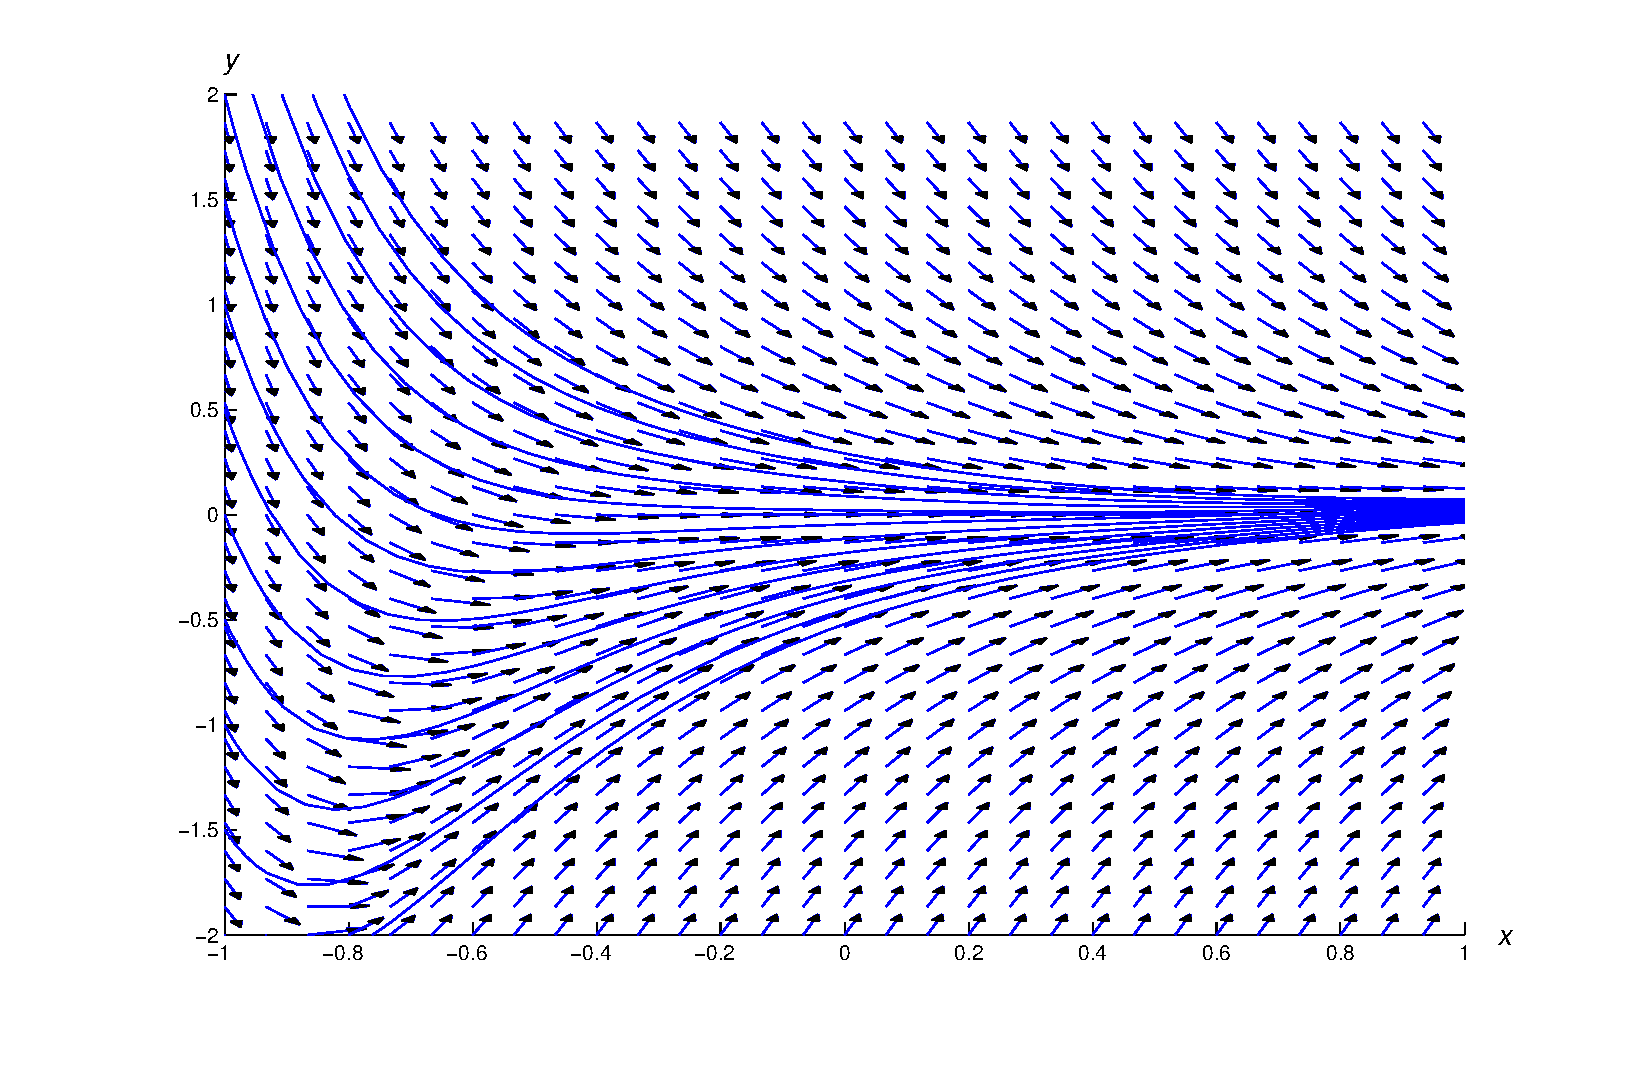
\includegraphics[bb=-78 148 689 643, width=5.67in, height=3.66in, keepaspectratio]{fig020103}
  \color{blue}
  \caption{A direction field and integral curves for $y'+2y=x^{3}e^{-2x}$}
  \label{figure:2.1.3}
\end{figure}
\end{examplesolution}

\begin{example}
  \label{example:2.1.6}\rm\mbox{}%\newline
  \begin{alist}
    \item % (a)
    Find the general solution
    of \begin{equation}
      \label{eq:2.1.20}y'+(\cot x)y=x\csc x.
    \end{equation}

    \item % (b)
    Solve the initial value problem
    \begin{equation}
      \label{eq:2.1.21}y'+(\cot x)y=x\csc x,\quad y(\pi/2)=1.
    \end{equation}
  \end{alist}
\end{example}

\begin{examplesolution}
\solutionpart{a} Here $p(x)=\cot x$ and $f(x)=x\csc x$ are both continuous except at the points
$x=r\pi$, where $r$ is an integer. Therefore we seek solutions of \eqref{eq:2.1.20} on the intervals
$\left(r\pi,(r+1)\pi\right)$. We need a nontrivial solution $y_{1}$ of the complementary equation;
thus, $y_{1}$ must satisfy $y_{1}'+(\cot x)y_{1}=0$, which we rewrite as
\begin{equation}
  \label{eq:2.1.22}\frac{y_{1}'}{y_{1}}=-\cot x=-\frac{\cos x}{\sin x}.
\end{equation}
Integrating this yields
\[
  \ln|y_{1}|=-\ln|\sin x|,
\]
where we take the constant of integration to be zero since we need only {\color{blue}\it one\/}
function that satisfies \eqref{eq:2.1.22}. Clearly $y_{1}=1/\sin x$ is a suitable choice. Therefore
we seek solutions of \eqref{eq:2.1.20} in the form
\[
  y=\frac{u}{\sin x},
\]
so that
\begin{equation}
  \label{eq:2.1.23}y'=\frac{u'}{\sin x}-\frac{u\cos x}{\sin^{2}x}
\end{equation}
and
\begin{equation}
  \label{eq:2.1.24}
  \begin{array}{rcl}
    y'+(\cot x)y & = & \dst\frac{u'}{\sin x}-\dst\frac{u\cos x}{\sin^{2}x}+\dst\frac{u\cot x}{\sin x}    \\[2\jot]
                 & = & \dst\frac{u'}{\sin x}-\dst\frac{u\cos x}{\sin^{2}x}+\dst\frac{u\cos x}{\sin^{2}x} \\[2\jot]
                 & = & \dst\frac{u'}{\sin x}.
  \end{array}
\end{equation}
Therefore $y$ is a solution of \eqref{eq:2.1.20} if and only if
\[
  u'/\sin x=x\csc x=x/\sin x\mbox{\quad or, equivalently, \quad}u'=x.
\]
Integrating this yields
\begin{equation}
  \label{eq:2.1.25}u=\frac{x^{2}}{2}+c,\text{\quad and \quad }y=\frac{u}{\sin x}=\frac{x^{2}}{2\sin x}+\frac{c}{\sin x}
\end{equation}
is the general solution of \eqref{eq:2.1.20} on every interval $\left(r\pi,(r+1)\pi\right)$
($r=$integer).

\solutionpart{b} Imposing the initial condition $y(\pi/2)=1$ in \eqref{eq:2.1.25} yields
\[
  1=\frac{\pi^{2}}{8}+c\mbox{\quad or\quad}c=1-\frac{\pi^{2}}{8}.
\]
Thus,
\[
  y=\frac{x^{2}}{2\sin x}+\frac{(1-\pi^{2}/8)}{\sin x}
\]
is a solution of \eqref{eq:2.1.21}. The interval of validity of this solution is $(0,\pi)$;
Figure~\ref{figure:2.1.4} shows its graph.

\begin{figure}[H]
  \centering
  \scalebox{.8}{
  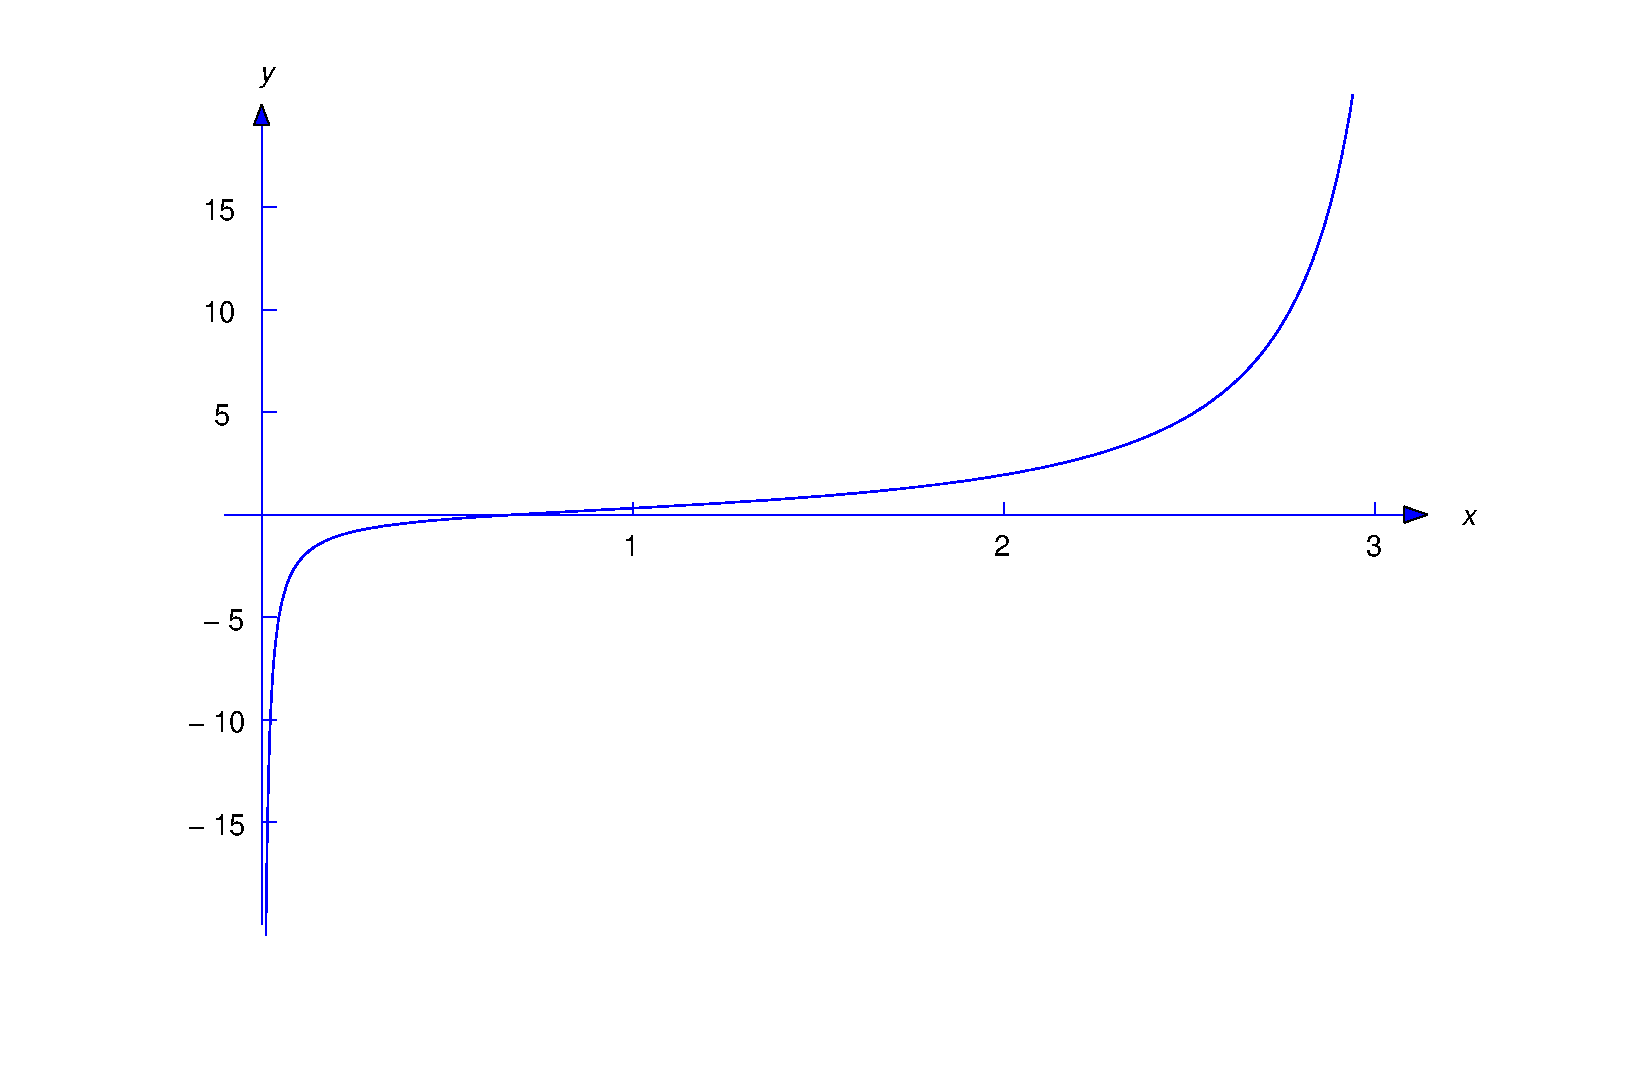
\includegraphics[bb=-78 148 689 643, width=5.67in, height=3.66in, keepaspectratio]{fig020104}}
  \color{blue}
  \caption{Solution of $y'+(\cot x)y=x\csc x$, $y(\pi/2)=1$}
  \label{figure:2.1.4}
\end{figure}

\color{blue}
\remark{It wasn't necessary to do the computations \eqref{eq:2.1.23} and \eqref{eq:2.1.24} in
Example~\ref{example:2.1.6}, since we showed in the discussion preceding Example~\ref{example:2.1.5}
that if $y=uy_{1}$ where $y_{1}'+p(x)y_{1}=0$, then $y'+p(x)y=u'y_{1}$. We did these computations so
you would see this happen in this specific example. We recommend that you include these
``unnecessary'' computations in doing exercises, until you're confident that you really understand
the method. After that, omit them.}
\color{black}
\end{examplesolution}

\medskip

We summarize the method of variation of parameters for solving

\begin{equation}
  \label{eq:2.1.26}y'+p(x)y=f(x)
\end{equation}
as follows:

\medskip
\color{blue}
\begin{alist}
  \item % (a)
  Find a function $y_{1}$ such that
  \[
    \frac{y_{1}'}{y_{1}}=-p(x).
  \]
  For convenience, take the constant of integration to be zero.

  \item % (b)
  Write
  \begin{equation}
    \label{eq:2.1.27}y=uy_{1}
  \end{equation}
  to remind yourself of what you're doing.

  \item % (c)
  Write $u'y_{1}=f$ and solve for $u'$; thus, $u'=f/y_{1}$.

  \item % (d
  Integrate $u'$ to obtain $u$, with an arbitrary constant of integration.

  \item % (e)
  Substitute $u$ into \eqref{eq:2.1.27} to obtain $y$.
\end{alist}
\color{black}

\medskip
To solve an equation written as
\[
  P_{0}(x)y'+P_{1}(x)y=F(x),
\]
we recommend that you divide through by $P_{0}(x)$ to obtain an equation of the form
\eqref{eq:2.1.26} and then follow this procedure.

\boxit{Solutions in Integral Form}

\noindent
Sometimes the integrals that arise in solving a linear first order equation can't be evaluated in
terms of elementary functions. In this case the solution must be left in terms of an integral.

\begin{example}
  \label{example:2.1.7}\rm \mbox{}
  \newline
  \begin{alist}
    \item % (a)
    Find the general solution of
    \[
      y'-2xy=1.
    \]

    \item % (b)
    Solve the initial value problem
    \begin{equation}
      \label{eq:2.1.28}y'-2xy=1,\quad y(0)=y_{0}.
    \end{equation}
  \end{alist}
\end{example}

\begin{examplesolution}
\solutionpart{a} To apply variation of parameters, we need a nontrivial solution $y_{1}$ of the
complementary equation; thus, $y_{1}'-2xy_{1}=0$, which we rewrite as
\[
  \frac{y_{1}'}{y_{1}}=2x.
\]
Integrating this and taking the constant of integration to be zero yields
\[
  \ln|y_{1}|=x^{2},\mbox{\quad so \quad}|y_{1}|=e^{x^{2}}.
\]
We choose $y_{1}=e^{x^{2}}$ and seek solutions of \eqref{eq:2.1.28} in the form $y=ue^{x^{2}}$,
where
\[
  u'e^{x^{2}}=1,\mbox{\quad so \quad}u'=e^{-x^{2}}.
\]
Therefore
\[
  u=c+\int e^{-x^{2}}dx,
\]
but we can't simplify the integral on the right because there's no elementary function with
derivative equal to $e^{-x^{2}}$. Therefore the best available form for the general solution of
\eqref{eq:2.1.28} is
\begin{equation}
  \label{eq:2.1.29}y=ue^{x^{2}}=e^{x^{2}}\left(c+\int e^{-x^{2}}dx\right).
\end{equation}

\solutionpart{b} Since the initial condition in \eqref{eq:2.1.28} is imposed at $x_{0}=0$, it is
convenient to rewrite \eqref{eq:2.1.29} as
\[
  y=e^{x^{2}}\left(c+\int^{x}_{0}e^{-t^{2}}dt\right),\mbox{\quad since \quad}\int_{0}^{0}e^{-t^{2}}\,dt=0.
\]
Setting $x=0$ and $y=y_{0}$ here shows that $c=y_{0}$. Therefore the solution of the initial value
problem is
\begin{equation}
  \label{eq:2.1.30}y=e^{x^{2}}\left(y_{0}+\int^{x}_{0}e^{-t^{2}}dt\right).
\end{equation}
For a given value of $y_{0}$ and each fixed $x$, the integral on the right can be evaluated by
numerical methods. An alternate procedure is to apply the numerical integration procedures discussed
in Chapter~3 directly to the initial value problem \eqref{eq:2.1.28}. Figure~\ref{figure:2.1.5}
shows graphs of \eqref{eq:2.1.30} for several values of $y_{0}$.

\begin{figure}[H]
  \centering
  \scalebox{.9}{
  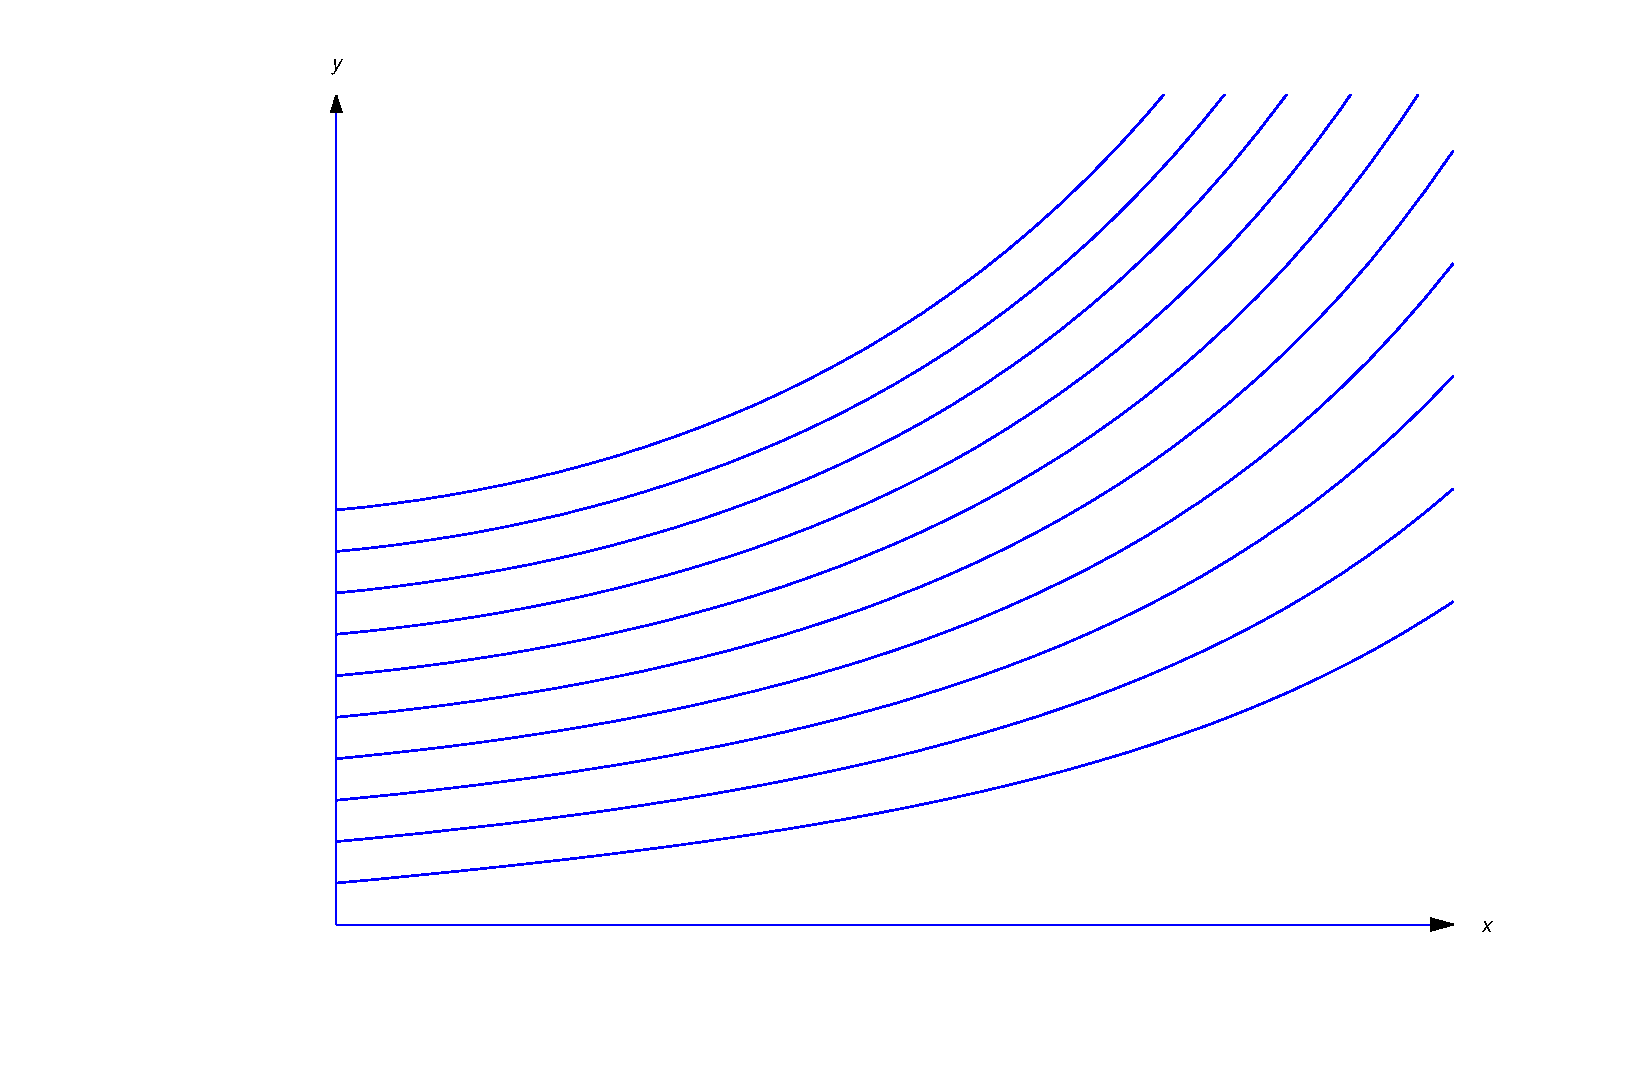
\includegraphics[bb=-78 148 689 643, width=5.67in, height=3.66in, keepaspectratio]{fig020105}
  }
  \color{blue}
  \caption{Solutions of $y'-2xy=1$, $y(0)=y_{0}$}
  \label{figure:2.1.5}
\end{figure}
\end{examplesolution}

\boxit{An Existence and Uniqueness Theorem}

\noindent
The method of variation of parameters leads to this theorem.

\begin{theorem}
  \color{blue}
  \label{thmtype:2.1.2} Suppose $p$ and $f$ are continuous on an open interval $(a,b)$, and let
  $y_{1}$ be any nontrivial solution of the complementary equation
  \[
    y'+p(x)y=0
  \]
  on $(a,b)$. Then:
  \begin{alist}
    \item % (a)
    The general solution of the nonhomogeneous equation
    \begin{equation}
      \label{eq:2.1.31}y'+p(x)y=f(x)
    \end{equation}
    on $(a,b)$ is
    \begin{equation}
      \label{eq:2.1.32}y=y_{1}(x)\left(c+\int f(x)/y_{1}(x)\,dx\right).
    \end{equation}

    \item % (b)
    If $x_{0}$ is an arbitrary point in $(a,b)$ and $y_{0}$ is an arbitrary real number, then the
    initial value problem
    \[
      y'+p(x)y=f(x),\quad y(x_{0})=y_{0}
    \]
    has the unique solution
    \[
      y=y_{1}(x)\left(\frac{y_{0}}{y_{1}(x_{0})}+\int^{x}_{x_{0}}\frac{f(t)}{y_{1}(t)}\,dt\right)
    \]
    on $(a,b)$.
  \end{alist}
\end{theorem}

\proof \part{a} To show that \eqref{eq:2.1.32} is the general solution of \eqref{eq:2.1.31} on
$(a,b)$, we must prove that:

\begin{rmlist}
  \item % (i)
  If $c$ is any constant, the function $y$ in \eqref{eq:2.1.32} is a solution of \eqref{eq:2.1.31}
  on $(a,b)$.

  \item % (ii)
  If $y$ is a solution of \eqref{eq:2.1.31} on $(a,b)$ then $y$ is of the form \eqref{eq:2.1.32} for
  some constant~$c$.
\end{rmlist}

To prove \part{i}, we first observe that any function of the form \eqref{eq:2.1.32} is defined on
$(a,b)$, since $p$ and $f$ are continuous on $(a,b)$. Differentiating \eqref{eq:2.1.32} yields
\[
  y'=y_{1}'(x)\left(c+\int f(x)/y_{1}(x)\, dx\right)+f(x).
\]
Since $y_{1}'=-p(x)y_{1}$, this and \eqref{eq:2.1.32} imply that
\begin{eqnarray*}
  y' & = & -p(x)y_{1}(x)\left(c+\int f(x)/y_{1}(x)\,dx\right)+f(x) \\
     & = & -p(x)y(x)+f(x),
\end{eqnarray*}
which implies that $y$ is a solution of \eqref{eq:2.1.31}.

To prove \part{ii}, suppose $y$ is a solution of \eqref{eq:2.1.31} on $(a,b)$. From the proof of
Theorem~\ref{thmtype:2.1.1}, we know that $y_{1}$ has no zeros on $(a,b)$, so the function
$u=y/y_{1}$ is defined on $(a,b)$. Moreover, since
\[
  y'=-py+f\mbox{\quad and\quad}y_{1}'=-py_{1},
\]
\begin{eqnarray*}
  u' & = & \frac{y_{1}y'-y_{1}'y}{y_{1}^{2}} \\[2\jot]
     & = & \frac{y_{1}(-py+f)-(-py_{1})y}{y_{1}^{2}}=\frac{f}{y_{1}}.
\end{eqnarray*}
Integrating $u'=f/y_{1}$ yields
\[
  u=\left(c+\int f(x)/y_{1}(x)\,dx\right),
\]
which implies \eqref{eq:2.1.32}, since $y=uy_{1}$.

\part{b} We've proved \part{a}, where $\int f(x)/y_{1}(x)\,dx$ in \eqref{eq:2.1.32} is an arbitrary
antiderivative of $f/y_{1}$. Now it's convenient to choose the antiderivative that equals zero when
$x=x_{0}$, and write the general solution of \eqref{eq:2.1.31} as
\[
  y=y_{1}(x)\left(c+\int^{x}_{x_{0}}\frac{f(t)}{y_{1}(t)}\,dt\right).
\]
Since
\[
  y(x_{0})=y_{1}(x_{0})\left(c+\int^{x_{0}}_{x_{0}}\frac{f(t)}{y_{1}(t)}\,dt\right)=cy_{1}(x_{0}),
\]
we see that $y(x_{0})=y_{0}$ if and only if $c=y_{0}/y_{1}(x_{0})$.

\exercises In Exercises~\ref{exer:2.1.1}--\ref{exer:2.1.5} find the general solution.

\begin{exerciselist}
  \begin{tabular}[t]{@{}p{168pt}@{}p{168pt}}
    \item\label{exer:2.1.1} $y'+ay=0$ ($a$=constant) &
    \item\label{exer:2.1.2}\vspace*{10pt} $y'+3x^{2}y=0$
  \end{tabular}

  \begin{tabular}[t]{@{}p{168pt}@{}p{168pt}}
    \item\label{exer:2.1.3} $xy'+(\ln x)y=0$ &
    \item\label{exer:2.1.4} $xy'+3y=0$
  \end{tabular}

  \begin{tabular}[t]{@{}p{168pt}@{}p{168pt}}
    \item\label{exer:2.1.5} $x^{2}y'+y=0$ &
  \end{tabular}

  \exercisetext{In Exercises~\ref{exer:2.1.6}--\ref{exer:2.1.11} solve the initial value problem.}

  \item\label{exer:2.1.6} $\dst{y'+\left(\frac{1+x}{x}\right)y=0,\quad y(1)=1}$

  \item\label{exer:2.1.7} $\dst{xy'+\left(1+\frac{1}{\ln x}\right)y=0,\quad y(e)=1}$

  \item\label{exer:2.1.8} $\dst{xy'+(1+x\cot x)y=0,\quad y\left(\frac{\pi}{2} \right)=2}$

  \item\label{exer:2.1.9} $\dst{y'-\left(\frac{2x}{1+x^{2}}\right)y=0,\quad y(0)=2}$

  \item\label{exer:2.1.10} $\dst{y'+\frac{k}{x}y=0,\quad y(1)=3 \quad\mbox{($k$= constant)}}$

  \item\label{exer:2.1.11} $\dst y'+(\tan kx)y=0,\quad y(0)=2 \quad\mbox{($k=$ constant)}$

  \exercisetext{In Exercises~\ref{exer:2.1.12} --\ref{exer:2.1.15} find the general solution. Also,
  plot a direction field and some integral curves on the rectangular region
  $\{-2\le x\le2,\ -2\le y\le2$\}.}

  \begin{tabular}{@{}p{168pt}@{}p{168pt}}
    \item\label{exer:2.1.12} \CGex $y'+3y=1$ &
    \item\label{exer:2.1.13}\vspace*{6pt} \CGex $\dst{y'+\left(\frac{1}{x}- 1\right)y=-\frac{2}{x}}$
  \end{tabular}

  \begin{tabular}{@{}p{168pt}@{}p{168pt}}
    \item\label{exer:2.1.14} \CGex $y'+2xy=xe^{-x^{2}}$ &
    \item\label{exer:2.1.15} \CGex $\dst{y'+\frac{2x}{1+x^{2}}y=\frac{e^{-x}}{1+x^{2}}}$
  \end{tabular}

  \exercisetext{In Exercises~\ref{exer:2.1.16} --\ref{exer:2.1.24} find the general solution.}

  \begin{tabular}[t]{@{}p{168pt}@{}p{168pt}}
    \item\label{exer:2.1.16} $\dst{y'+\frac{1}{x}y=\frac{7}{x^{2}}+3}$ &
    \item\label{exer:2.1.17}\vspace*{8pt} $\dst{y'+\frac{4}{x-1}y =\frac{1}{(x-1)^{5}}+\frac{\sin x}{(x-1)^{4}}}$
  \end{tabular}

  \begin{tabular}[t]{@{}p{168pt}@{}p{168pt}}
    \item\label{exer:2.1.18} $xy'+(1+2x^{2})y=x^{3}e^{-x^{2}}$ &
    \item\label{exer:2.1.19}\vspace*{-8pt} $\dst{xy'+2y=\frac{2}{x^{2}}+1}$
  \end{tabular}

  \begin{tabular}[t]{@{}p{168pt}@{}p{168pt}}
    \item\label{exer:2.1.20} $y'+(\tan x)y=\cos x$ &
    \item\label{exer:2.1.21}\vspace*{-5pt} $\dst{(1+x)y'+2y=\frac{\sin x}{1+x}}$
  \end{tabular}

  \item\label{exer:2.1.22} $(x-2)(x-1)y'-(4x-3)y=(x-2)^{3}$

  \begin{tabular}[t]{@{}p{168pt}@{}p{168pt}}
    \item\label{exer:2.1.23} $y'+(2\sin x\cos x)y=e^{-\sin^{2}x}$ &
    \item\label{exer:2.1.24} $x^{2}y'+3xy=e^{x}$
  \end{tabular}

  \exercisetext{In Exercises~\ref{exer:2.1.25}--\ref{exer:2.1.29} solve the initial value problem
  and sketch the graph of the solution.}

  \item\label{exer:2.1.25} \CGex $y'+7y=e^{3x},\quad y(0)=0$

  \item\label{exer:2.1.26} \CGex $\dst{(1+x^{2})y'+4xy=\frac{2}{1+x^{2}},\quad y(0)=1}$

  \item\label{exer:2.1.27} \CGex $\dst{xy'+3y=\frac{2}{x(1+x^{2})},\quad y(-1)=0}$

  \item\label{exer:2.1.28} \CGex $\dst{y'+(\cot x)y=\cos x,\quad y\left(\frac{\pi}{2}\right)=1}$

  \item\label{exer:2.1.29} \CGex $\dst{y'+\frac{1}{x}y=\frac{2}{x^{2}}+1,\quad y(-1)=0}$

  \exercisetext{In Exercises~\ref{exer:2.1.30}--\ref{exer:2.1.37} solve the initial value problem.}

  \item\label{exer:2.1.30}
        $\dst{(x-1)y'+3y=\frac{1}{(x-1)^{3}}+ \frac{\sin x}{(x-1)^{2}},\quad y(0)=1}$

  \item\label{exer:2.1.31} $xy'+2y=8x^{2},\quad y(1)=3$

  \item\label{exer:2.1.32} $xy'-2y=-x^{2},\quad y(1)=1$

  \item\label{exer:2.1.33} $y'+2xy=x,\quad y(0)=3$

  \item\label{exer:2.1.34} $\dst{(x-1)y'+3y=\frac{1+(x-1)\sec^{2}x}{(x-1)^{3}},\quad y(0)=-1}$

  \item\label{exer:2.1.35} $\dst{(x+2)y'+4y=\frac{1+2x^{2}}{x(x+2)^{3}},\quad y(-1)=2}$

  \item\label{exer:2.1.36} $(x^{2}-1)y'-2xy=x(x^{2}-1),\quad y(0)=4$

  \item\label{exer:2.1.37} $(x^{2}-5)y'-2xy=-2x(x^{2}-5),\quad y(2)=7$

  \exercisetext{In Exercises~\ref{exer:2.1.38}--\ref{exer:2.1.42} solve the initial value problem
  and leave the answer in a form involving a definite integral. (You can solve these problems
  numerically by methods discussed in Chapter~3.)}

  \item\label{exer:2.1.38} $y'+2xy=x^{2},\quad y(0)=3$

  \item\label{exer:2.1.39} $\dst{y'+\frac{1}{x}y=\frac{\sin x}{x^{2}},\quad y(1)=2}$

  \item\label{exer:2.1.40} $\dst{y'+y=\frac{e^{-x}\tan x}{x},\quad y(1)=0}$

  \item\label{exer:2.1.41} $\dst{y'+\frac{2x}{1+x^{2}}y=\frac{e^{x}}{(1+x^{2})^{2}},\quad y(0)=1}$

  \item\label{exer:2.1.42} $xy'+(x+1)y=e^{x^{2}},\quad y(1)=2$

  \item\label{exer:2.1.43}

  Experiments indicate that glucose is absorbed by the body at a rate proportional to the amount of
  glucose present in the bloodstream. Let $\lambda$ denote the (positive) constant of
  proportionality. Now suppose glucose is injected into a patient's bloodstream at a constant rate
  of $r$ units per unit of time. Let $G=G(t)$ be the number of units in the patient's bloodstream at
  time $t>0$. Then
  \[
    G'=-\lambda G+r,
  \]
  where the first term on the right is due to the absorption of the glucose by the patient's body
  and the second term is due to the injection. Determine $G$ for $t>0$, given that $G(0)=G_{0}$.
  Also, find $\lim_{t\to\infty}G(t)$.

  \item\label{exer:2.1.44}
  \begin{alist}
    \item % (a)
    \Lex Plot a direction field and some integral curves for
    \[
      xy'-2y=-1 \eqno{\rm(A)}
    \]
    on the rectangular region $\{-1\le x\le1,-.5\le y\le1.5\}$. What do all the integral curves have
    in common?

    \item % (b)
    Show that the general solution of (A) on $(-\infty,0)$ and $(0,\infty)$ is
    \[
      y=\frac{1}{2}+cx^{2}.
    \]

    \item % (c)
    Show that $y$ is a solution of (A) on $(-\infty,\infty)$ if and only if
    \[
      y=\left\{
      \begin{array}{ll}
        \dst{\frac{1}{2}+c_{1}x^{2}}, & x \ge0, \\[2\jot]
        \dst{\frac{1}{2}+c_{2}x^{2}}, & x<0,
      \end{array}\right.
    \]
    where $c_{1}$ and $c_{2}$ are arbitrary constants.

    \item % (c)
    Conclude from \part{c} that all solutions of (A) on $(-\infty,\infty)$ are solutions of the
    initial value problem
    \[
      xy'-2y=-1,\quad y(0)=\frac{1}{2}.
    \]

    \item % (d)
    Use \part{b} to show that if $x_{0}\ne0$ and $y_{0}$ is arbitrary, then the initial value
    problem
    \[
      xy'-2y=-1,\quad y(x_{0})=y_{0}
    \]
    has infinitely many solutions on ($-\infty,\infty$). Explain why this doesn't contradict
    Theorem~\ref{thmtype:2.1.2}\part{b}.
  \end{alist}

  \item\label{exer:2.1.45} Suppose $f$ is continuous on an open interval $(a,b)$ and $\alpha$ is a
        constant.
  \begin{alist}
    \item % (a)
    Derive a formula for the solution of the initial value problem
    \renewcommand{\theequation}{\Alph{equation}}
    \[
      y'+\alpha y=f(x),\quad y(x_{0})=y_{0}, \eqno{\rm(A)}
    \]
    where $x_{0}$ is in $(a,b)$ and $y_{0}$ is an arbitrary real number.

    \item % (b)
    Suppose $(a,b)=(a,\infty)$, $\alpha>0$ and $\displaystyle{\lim_{x\to\infty}f(x)=L}$. Show that
    if $y$ is the solution of (A), then $\displaystyle{\lim_{x\to \infty}y(x)=L/\alpha}$.
  \end{alist}

  \item\label{exer:2.1.46} Assume that all functions in this exercise are defined on a common
        interval $(a,b)$.
  \begin{alist}
    \item % (a)
    Prove: If $y_{1}$ and $y_{2}$ are solutions of
    \[
      y'+p(x)y=f_{1}(x)
    \]
    and
    \[
      y'+p(x)y=f_{2}(x)
    \]
    respectively, and $c_{1}$ and $c_{2}$ are constants, then $y=c_{1}y_{1}+c_{2}y_{2}$ is a
    solution of
    \[
      y'+p(x)y=c_{1}f_{1}(x)+c_{2}f_{2}(x).
    \]
    (This is the {\it principle of superposition.\/})

    \item % (b)
    Use \part{a} to show that if $y_{1}$ and $y_{2}$ are solutions of the nonhomogeneous equation
    \[
      y'+p(x)y=f(x), \eqno{\rm(A)}
    \]
    then $y_{1}-y_{2}$ is a solution of the homogeneous equation
    \[
      y'+p(x)y=0. \eqno{\rm(B)}
    \]

    \item % (c)
    Use \part{a} to show that if $y_{1}$ is a solution of (A) and $y_{2}$ is a solution of (B), then
    $y_{1}+y_{2}$ is a solution of (A).
  \end{alist}

  \item\label{exer:2.1.47} Some nonlinear equations can be transformed into linear equations by
        changing the dependent variable. Show that if
  \[
    g'(y)y'+p(x)g(y)=f(x)
  \]
  where $y$ is a function of $x$ and $g$ is a function of $y$, then the new dependent variable
  $z=g(y)$ satisfies the linear equation
  \[
    z'+p(x)z=f(x).
  \]

  \item\label{exer:2.1.48} Solve by the method discussed in Exercise~\ref{exer:2.1.47}.

  \vspace*{6pt}
  \begin{tabular}[t]{@{}p{168pt}@{}p{168pt}}
    {\bf (a)} $(\sec^{2}y)y'-3\tan y=-1$ & {\bf (b)} $\dst{e^{y^{2}}\left(2yy'+ \frac{2}{x}\right)=\frac{1}{x^{2}}}$
  \end{tabular}

  \begin{tabular}[t]{@{}p{168pt}@{}p{168pt}}
    {\bf (c)} $\dst{\frac{xy'}{y}+2\ln y=4x^{2}}$ & {\bf (d)} $\dst{\frac{y'}{(1+y)^{2}}- \frac{1}{x(1+y)}=-\frac{3}{x^{2}}}$
  \end{tabular}

  \item\label{exer:2.1.49} We've shown that if $p$ and $f$ are continuous on $(a,b)$ then every
        solution of
  \[
    y'+p(x)y=f(x) \eqno{\rm(A)}
  \]
  on $(a,b)$ can be written as $y=uy_{1}$, where $y_{1}$ is a nontrivial solution of the
  complementary equation for (A) and $u'=f/y_{1}$. Now suppose $f$, $f'$, \dots, $f^{(m)}$ and $p$,
  $p'$, \dots, $p^{(m-1)}$ are continuous on $(a,b)$, where $m$ is a positive integer, and define
  \begin{eqnarray*}
    f_{0} & = & f, \\
    f_{j} & = & f_{j-1}'+pf_{j-1},\quad1\le j\le m.
  \end{eqnarray*}
  Show that
  \[
    u^{(j+1)}=\frac{f_{j}}{y_{1}},\quad0\le j\le m.
  \]
\end{exerciselist}
